\clearpage
\subsection{Implementation view}
\copied{The development view illustrates a system from a programmer's perspective and is concerned with software management. This view is also known as the implementation view. It uses the UML Component diagram to describe system components. UML Diagrams used to represent the development view include the Package diagram.}
{from wikipedia\\\url{https://en.wikipedia.org/wiki/4\%2B1_architectural_view_model}}

The implementation view, also known as the development view, describes the system from the programmer's perspective. This includes a description of the components of the system and how the system is packaged.  

\subsubsection{Components}
The system consists of a set of components tat all interact with each other. In figure~\ref{fig:component} below, these different components are shown. Each component can provide interfaces and uses sockets to connect to interfaces of other components. This way, the implementation of each component can independently be replaced and deployed. 

\clearpage
\begin{figure}[hb!]
%\centering
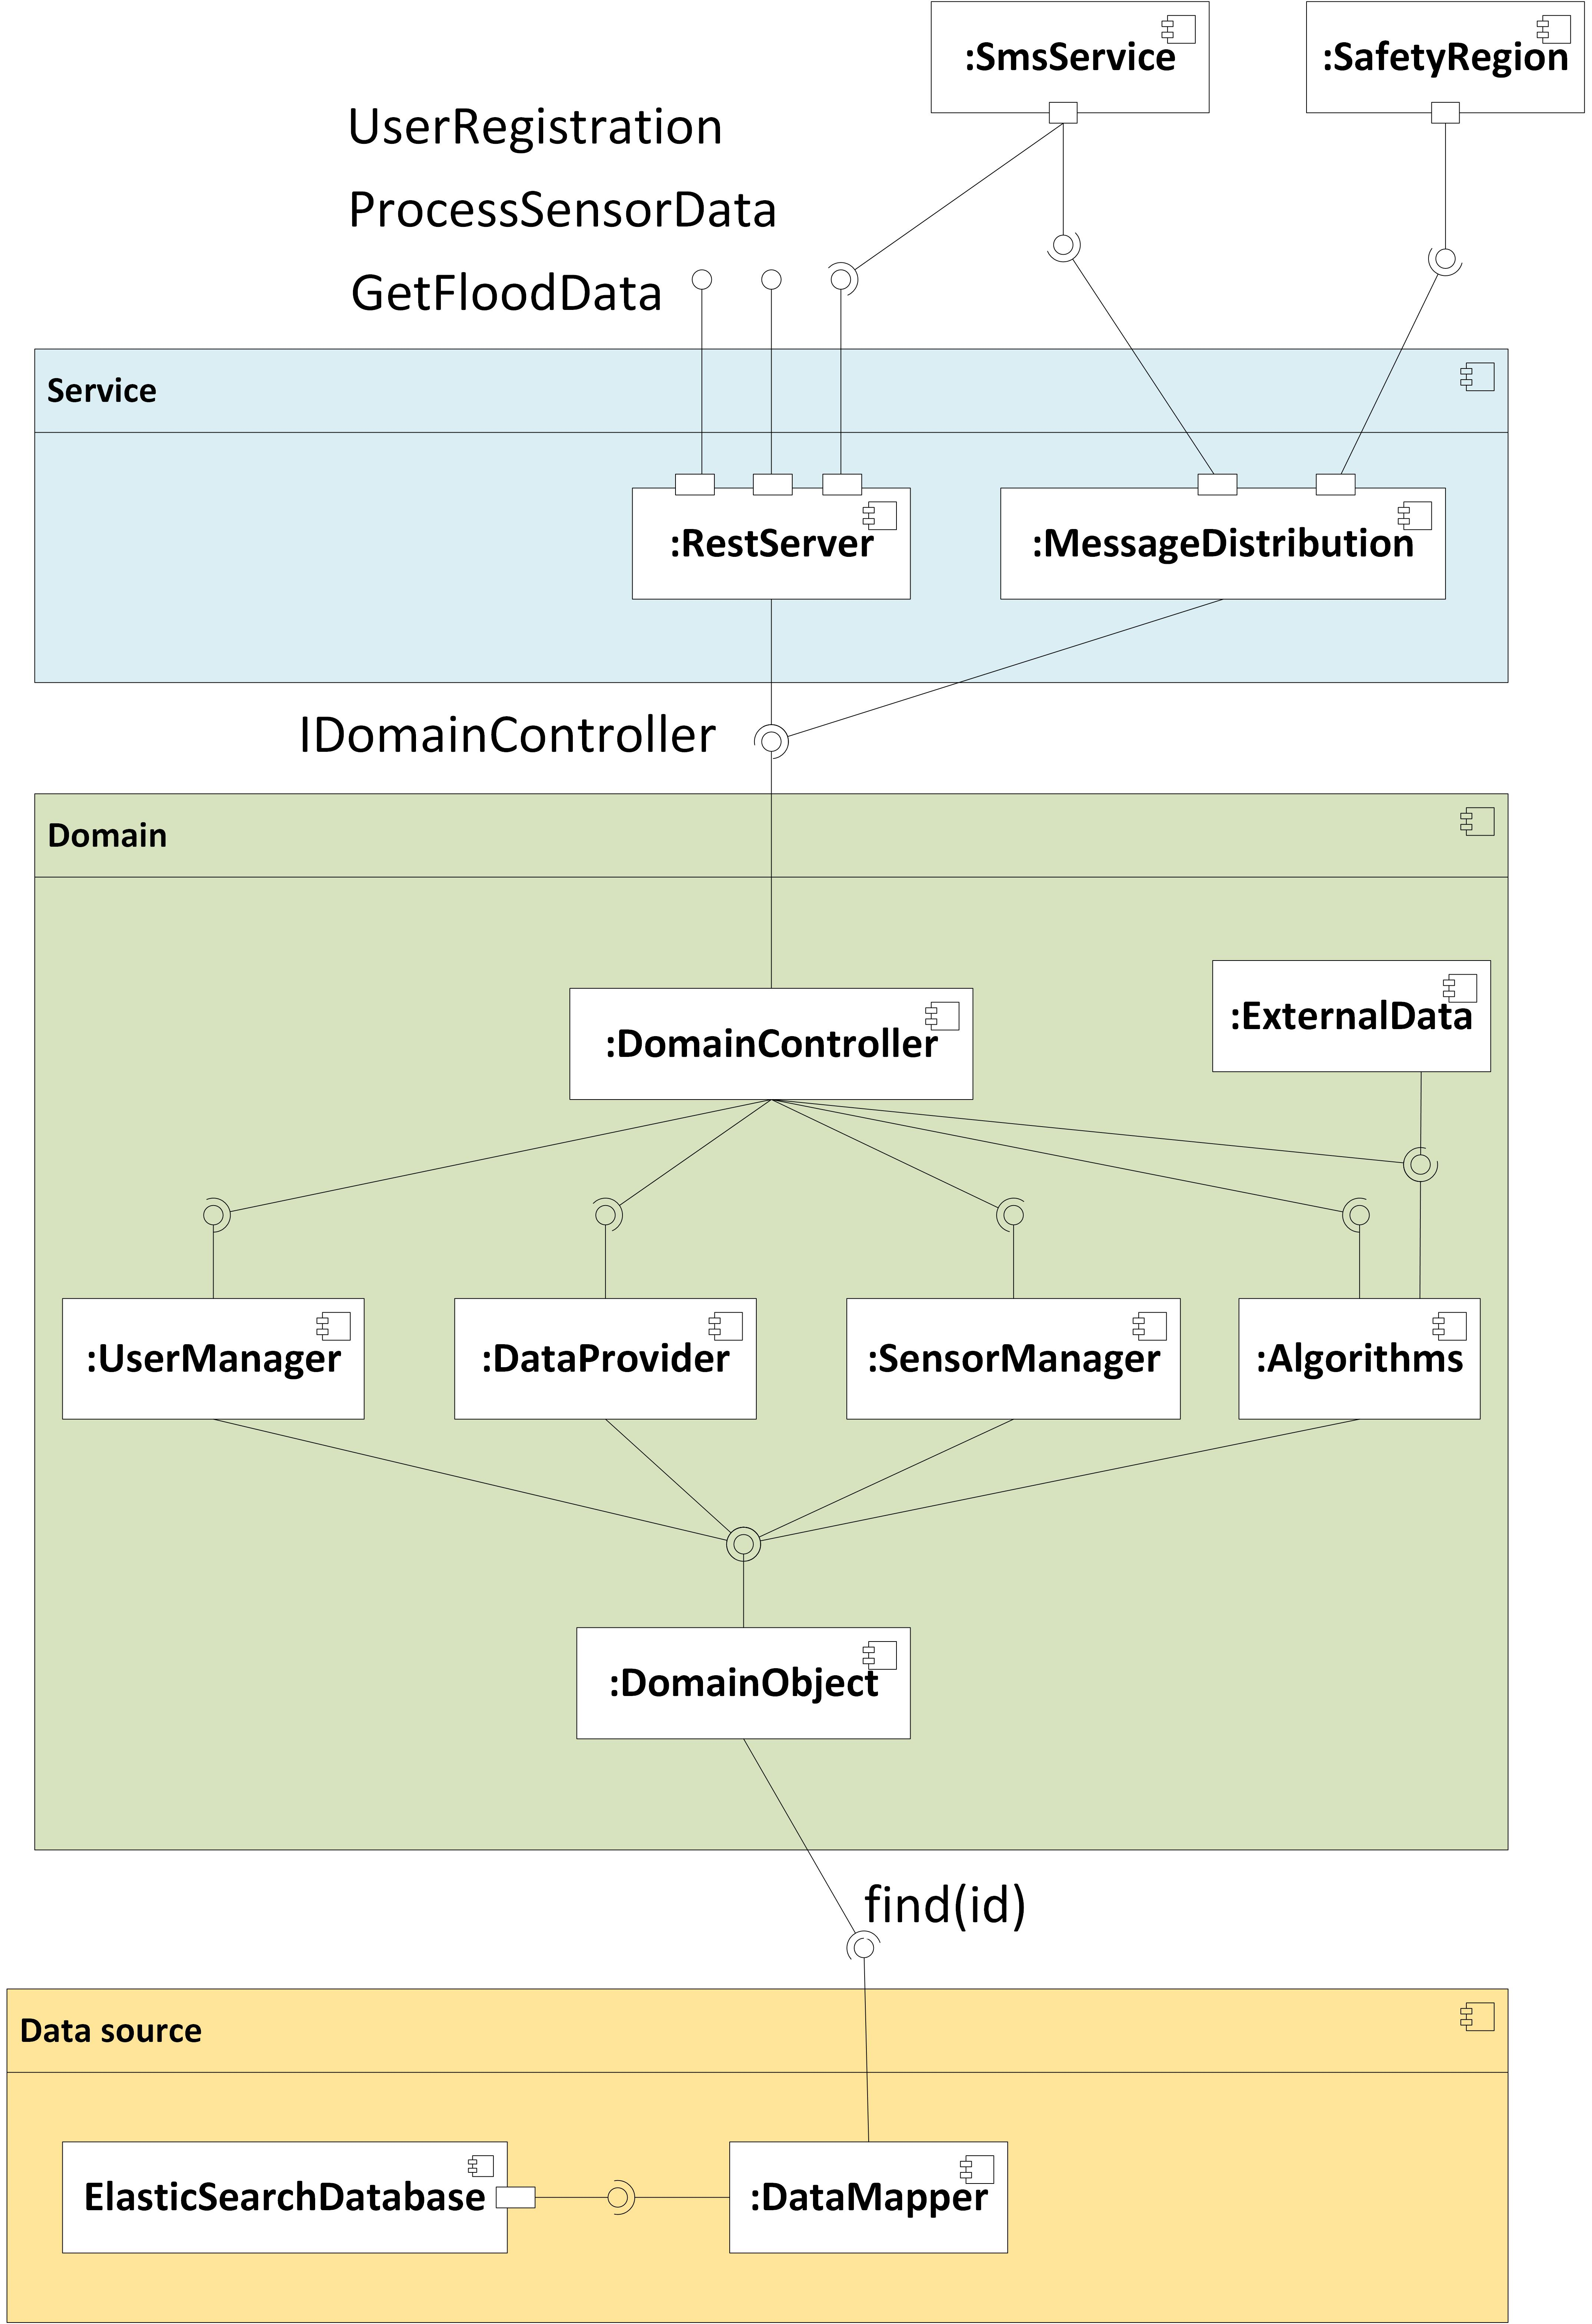
\includegraphics[keepaspectratio=true,height=13cm,width=0.9\textwidth]{{\viewimages/component}.jpg}
\caption{Component diagram}
\label{fig:component}
\end{figure}

The layering is done according to the layering Martin Fowler proposes for enterprise applications \cite{Fowler:2002:PEA:579257,Fowler:web:servicelayer}.
The data mapper \cite{Fowler:2002:PEA:579257} is used to completely separate and ignore the database in the domain model. This provides a more flexible architecture that allows modifications of either the database or the domain model independently without having to alter the other layer.
\subsubsection{Packages}
The software of the system is divided into several packages. These packages and their relations can be seen in figure~\ref{fig:package-diagram}. 
In this diagram, «use» depicts the use of an interface exposed by a software package, «access» depicts a private import of (parts of) another package, while «import» means a public import of (parts of) another package. 

The diagram contains software packages of the system itself, as well as software packages provided by third parties. The software packages provided by third parties are drawn outside of the `Smart Flood Monitoring System'-box.

\begin{figure}[hb!]
%\centering
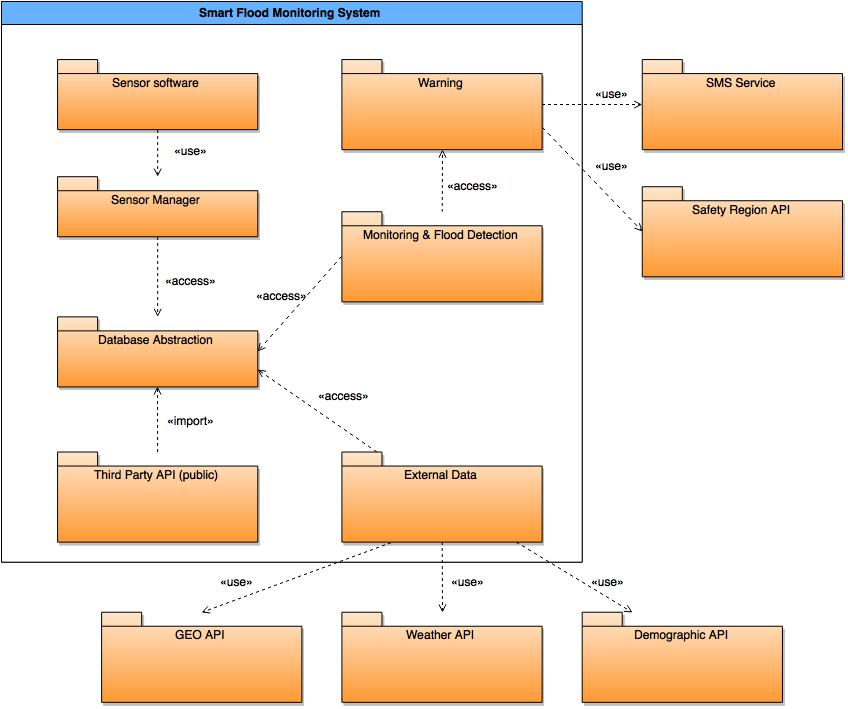
\includegraphics[keepaspectratio=true,width=1.0\textwidth]{{\viewimages/packages}.png}
\caption{Package diagram}
\label{fig:package-diagram}
\end{figure}

\subsubsection{Decisions}
\pgfplotstabletypeset[%
UCTable
]{%
	value & description \\
	Name & Data source architectural pattern \\
	Decision & \req{dec}\\
	Problem/Issue & The system components need to be abstract and individually replaceable without having to alter the entire system\\
	Decision & 	\compactCell{The data mapper \cite{Fowler:2002:PEA:579257} is used to completely separate and ignore the database in the domain model. This provides a more flexible architecture that allows modifications of either the database or the domain model independently without having to alter the other layer.}.\\
	Alternatives & Table data gateway, row gateway, active record \\
	Arguments & 	\compactCell{%
		\textbf{Table data gateway} The table data gateway is a pattern that, for each domain class, provides a gateway class. This gateway class proviedes methods to that do all the database interaction. This way all the SQL statements will be stored in the gateway class and thus is seperated from the domain layer.%
		\\
		\textbf{Row gateway} Same idea as the table data gateway, but now for individial rows, instead of a table.
		\\%
		\textbf{Active record} This is the most basic approach. In this pattern, the domain object also contains the logic of storing that object to the database.
	}\\
}